\documentclass{article}
\usepackage[top=1in, bottom=1in, left=1in, right=1in]{geometry}
\usepackage{graphicx}
\begin{document}

\begin{flushright}
Matt Jibson \\
EG 520 \\
HW 2
\end{flushright}

\begin{itemize}
	\item[7.2]
		\begin{itemize}
			\item[a] \ \\ 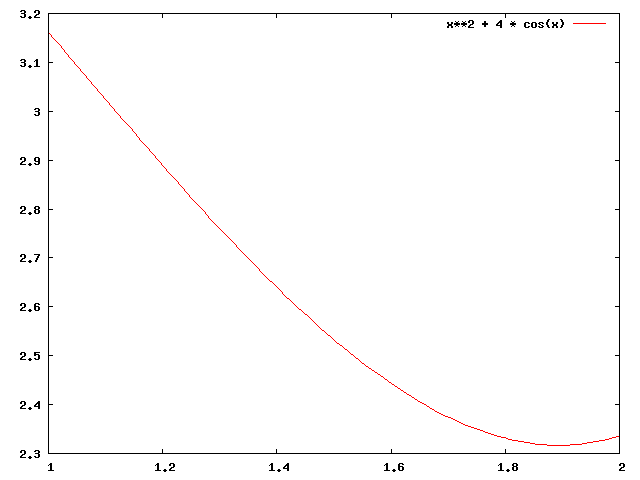
\includegraphics[width=0.5\linewidth]{72a.png}
			\item[b] $(0.61803)^N \le 0.2/1 \Rightarrow N = 4$. \\
				\begin{tabular}{cccccc}
					\hline
					Iteration $k$ & $a_k$ & $b_k$ & $f(a_k)$ & $f(b_k)$ & New uncertainty interval \\
					\hline
					1 & 1.38196601125 & 1.61803398875 & 2.66067058007 & 2.42915360373 & [1.38196601125, 2] \\
					2 & 1.61803398875 & 1.7639320225 & 2.42915360373 & 2.34370726837 & [1.61803398875, 2] \\
					3 & 1.7639320225 & 1.85410196625 & 2.34370726837 & 2.31956995865 & [1.7639320225, 2] \\
					4 & 1.85410196625 & 1.90983005625 & 2.31956995865 & 2.31714692162 & [1.85410196625, 2] \\
					\hline
				\end{tabular}
			\item[c]
		\end{itemize}
	\item[8.1]
	\item[8.3]
	\item[8.13]
	\item[8.17]
	\item[9.1]
	\item[9.3]
\end{itemize}

\end{document}